% ============================================================
\section{Evaluation}
\label{sec:evaluation}
% ============================================================

This section evaluates two tightly scoped contributions of \textsc{DeepTutor}.
First, we introduce a \textbf{student-centric benchmark and first-person interactive protocol} intended to measure tutoring quality from the learner's perspective rather than from the instructor's alone.
Second, we evaluate the \textbf{foundational tutoring pipeline}, including problem solving, question generation, and the shared personalization engine, which constitutes the experimentally validated core of the system.

We evaluate along three complementary axes.
\emph{First-person interactive evaluation}~(\S\ref{sec:interactive_eval}) probes adaptive personalization through simulated multi-turn student dialogues.
\emph{General problem-solving transfer}~(\S\ref{sec:generalization}) tests whether the tutoring-oriented pipeline decomposition strengthens the backbone's reasoning ability on standard benchmarks.
\emph{Component-level ablation}~(\S\ref{sec:ablation}) isolates the individual contribution of each architectural pillar.

% ===========================================================================
\subsection{TutorBench: A Student-Centric Benchmark}
\label{sec:tutorbench}
% ===========================================================================

Existing educational benchmarks predominantly adopt an instructor-centric perspective, treating the student as a generic receiver of instruction~\citep{chu-etal-2025-llm,kurdi2020systematic}.
\textsc{TutorBench} closes this gap: every entry couples a detailed learner persona with source-grounded knowledge gaps and an interactive tutoring task, placing the student at the center of evaluation.

\begin{figure*}[t]
  \centering
  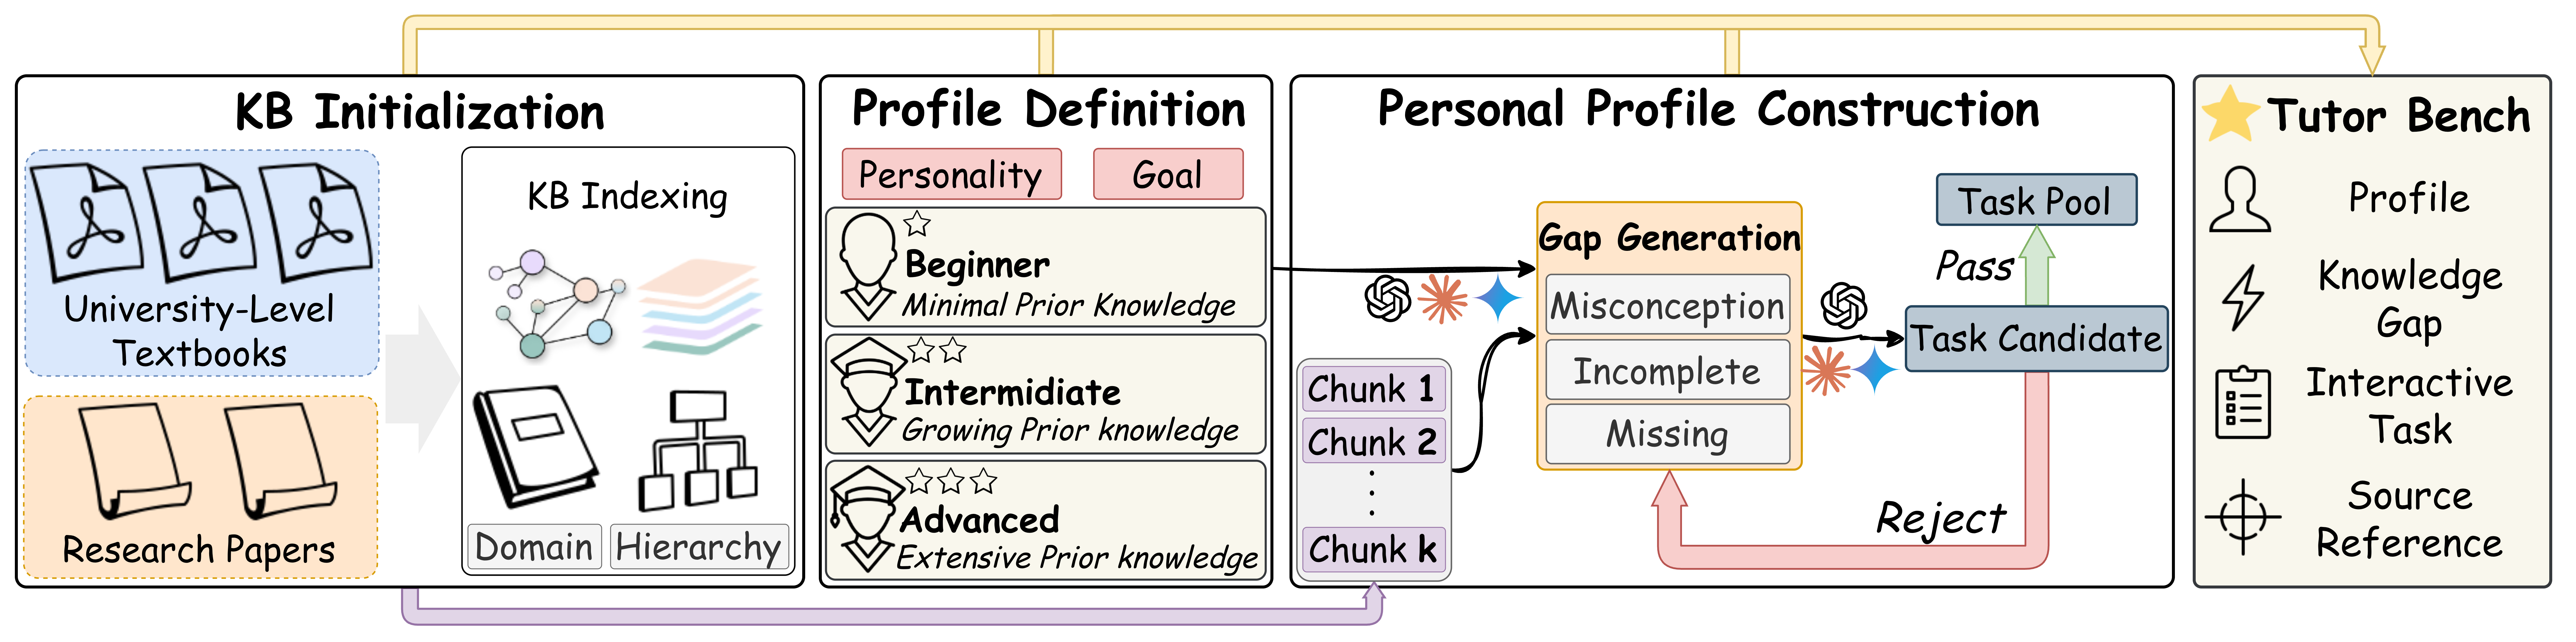
\includegraphics[width=\textwidth]{figures/bench-0315.png}
  \caption{Construction pipeline of \textsc{TutorBench}. Each entry contains a learner profile, source-grounded knowledge gaps, and an interactive tutoring task.}
  \label{fig:datagen}
\end{figure*}

\paragraph{Construction Pipeline.}
University-level textbooks and research papers are first indexed into the dual-representation knowledge base~(\S\ref{sec:rag}), from which a domain hierarchy is derived.
Each knowledge base instantiates three learner profiles at the \emph{beginner}, \emph{intermediate}, and \emph{advanced} levels, which differ in educational background, learning purpose, and per-topic mastery states.
For each profile, source-grounded knowledge gaps are generated across three types: \emph{misconceptions}, \emph{incomplete understanding}, and \emph{missing knowledge}~\citep{smith1993misconceptions,shute2008focus}.
These gaps are assembled into interactive tasks via rejection sampling that verifies gap coherence, task--gap alignment, and conversational naturalness.
All generated entries undergo human review for factual correctness, profile plausibility, and pedagogical soundness.

\paragraph{Statistics.}
\textsc{TutorBench} draws on 30 knowledge bases spanning five disciplines (humanities, sciences, engineering, business, and frontier research), instantiating 90 learner profiles and 270 interactive tasks.
Every entry carries three source-grounded knowledge gaps anchored to specific passages from the underlying materials.

% ===========================================================================
\subsection{First-Person Interactive Evaluation}
\label{sec:interactive_eval}
% ===========================================================================

Building on rubric-based LLM evaluation~\citep{zheng2023judging,huang2025mathtutorbench} and simulated-student paradigms~\citep{dinucujianu2025pedagogy,scarlatos2026simulatedstudents,pan2025tutorup}, we design a first-person interactive evaluation protocol (Figure~\ref{fig:evaluation}; Appendix~\ref{app:eval:simulator}) in which an LLM-based student simulator, initialized from a \textsc{TutorBench} entry with knowledge gaps rendered as first-person belief statements, engages each tutoring system in multi-turn dialogue.
The resulting transcripts are then scored by an independent LLM judge against personalized rubrics.

\paragraph{Metrics.}
Tutoring quality is assessed along ten dimensions, each scored on a 1--5 Likert scale.
Five \textbf{solve-side} metrics capture explanation quality: \emph{Source Faithfulness}~(SF), \emph{Personalization}~(PER), \emph{Applicability}~(APP), \emph{Vividness}~(VID), and \emph{Logical Depth}~(LD).
Five \textbf{practice-side} metrics capture question quality: \emph{Fitness}~(FIT), \emph{Groundedness}~(GND), \emph{Diversity}~(DIV), \emph{Answer Quality}~(ANS), and \emph{Cross Concept}~(CC).
Detailed rubric definitions appear in Appendix~\ref{app:eval:rubrics}.

\paragraph{Protocol.}
We use \emph{Gemini-3-Flash} to power both the student simulator and all tutor backbones, while \emph{Claude Sonnet~4.6} serves as the judge at temperature zero.
Each transcript is scored three times and averaged to reduce variance.
Results are obtained on the full \textsc{TutorBench} release consisting of 270 tasks across 90 profiles and 30 knowledge bases.

\paragraph{Baselines.}
To disentangle the contribution of our pipeline design from that of the backbone model, we construct four representative baselines within a unified evaluation harness that shares the same RAG tool and backbone:
\emph{Naive Tutor} (direct prompting),
\emph{CoT Tutor} (chain-of-thought~\citep{wei2022chain}),
\emph{Self-Refine Tutor} (draft followed by a pedagogical review pass~\citep{madaan2024selfrefine}), and
\emph{ReAct Tutor} (think--act--observe loop~\citep{yao2023reactsynergizingreasoningacting}).

{%
\setlength{\aboverulesep}{0pt}%
\setlength{\belowrulesep}{0pt}%
\renewcommand{\arraystretch}{1.18}%
\begin{table*}[t]
\centering
\small
\resizebox{\textwidth}{!}{%
\setlength{\tabcolsep}{4.2pt}
\begin{tabular}{l ccccc g ccccc g cc}
\toprule
& \multicolumn{6}{c}{\textbf{Solve Quality}}
& \multicolumn{6}{c}{\textbf{Practice Quality}}
& \multicolumn{2}{c}{\textbf{Overall}} \\
\cmidrule(lr){2-7} \cmidrule(lr){8-13} \cmidrule(lr){14-15}
\textbf{System}
  & SF & PER & APP & VID & LD & \textit{Avg}
  & FIT & GND & DIV & ANS & CC & \textit{Avg}
  & OQ & $\Delta$\% \\
\midrule
Naive Tutor
  & 3.22 & 4.24 & 4.44 & 3.89 & 3.99 & 3.96
  & 3.20 & 2.46 & 2.83 & 3.87 & 3.12 & 3.10
  & 3.53 & \textcolor{gray}{--} \\
CoT Tutor
  & 3.34 & 4.22 & 4.47 & 3.82 & 4.01 & 3.97
  & 3.18 & 2.50 & 2.79 & 3.81 & 3.04 & 3.06
  & 3.52 & {-0.28\%} \\
Self-Refine Tutor
  & 3.28 & 4.28 & \textbf{4.61} & 3.94 & 4.14 & 4.05
  & 3.17 & 2.49 & 2.88 & 3.88 & 2.97 & 3.08
  & 3.57 & {+1.13\%} \\
ReAct Tutor
  & \underline{3.35} & 4.37 & 4.40 & 3.70 & 3.96 & 3.96
  & 3.16 & 2.47 & 2.75 & \underline{3.94} & 3.07 & 3.08
  & 3.52 & {-0.28\%} \\
\midrule
\textsc{DeepTutor}
  & \textbf{3.36} & \textbf{4.59} & 4.56 & 4.81 & \textbf{4.61} & \textbf{4.39}
  & \textbf{3.35} & \textbf{2.96} & \textbf{3.44} & \textbf{3.98} & \textbf{3.38} & \textbf{3.42}
  & \textbf{3.91} & \textcolor{teal!80!black}{\textbf{+10.76\%}} \\
\quad w/o Memory
  & \textbf{3.36} & 4.22 & 4.57 & \textbf{4.83} & 4.52 & \underline{4.30}
  & 3.15 & \underline{2.80} & \underline{3.34} & 3.90 & \underline{3.31} & \underline{3.30}
  & \underline{3.80} & \textcolor{teal!80!black}{\textbf{+7.65\%}} \\
\quad w/o RAG
  & 3.11 & \underline{4.41} & 4.55 & \textbf{4.83} & \underline{4.53} & 4.29
  & \underline{3.31} & 2.23 & 3.30 & 3.84 & 3.19 & 3.17
  & 3.73 & \textcolor{teal!80!black}{\textbf{+5.67\%}} \\
\quad w/o RAG + Memory
  & 3.16 & 4.17 & \underline{4.60} & \underline{4.82} & 4.48 & 4.25
  & 3.25 & 2.22 & 3.27 & 3.85 & 3.14 & 3.15
  & 3.70 & \textcolor{teal!80!black}{\textbf{+4.82\%}} \\
\bottomrule
\end{tabular}}
\caption{Main results on \textsc{TutorBench}. Upper block: baselines. Lower block: \textsc{DeepTutor} with ablation variants. \textit{Avg}~is the group mean; OQ~is the \underline{O}verall \underline{Q}uality across all ten metrics; $\Delta$\%~is relative improvement over the Naive Tutor baseline. All metrics are 1--5~$\uparrow$. \textbf{Bold}~=~best; \underline{underline}~=~second best.}
\label{tab:interactive_all}
\end{table*}
}

\paragraph{Results.}
Table~\ref{tab:interactive_all} reveals a striking pattern: the four baselines cluster within a narrow performance band despite employing substantially different reasoning strategies, suggesting that reasoning sophistication alone does not translate into better personalization.
\textsc{DeepTutor} breaks out of this band, achieving an overall quality improvement of 10.76\% over the strongest baseline.

On the solve side, \emph{Vividness} sees the largest lift (+0.87 over the best baseline), reflecting the multi-stage pipeline's ability to produce structurally richer explanations with embedded examples and visual cues.
\emph{Personalization} and \emph{Logical Depth} follow, indicating that the system successfully diagnoses individual gaps and scaffolds logically grounded reasoning chains.
On the practice side, the advantage is even more pronounced.
\emph{Groundedness} records the largest absolute gain, benefiting directly from RAG-grounded question generation, while \emph{Diversity} and \emph{Cross Concept} profit from the structured learner history that guides the idea agent toward novel angles and inter-concept connections.

\paragraph{Cross-Domain Generalization.}
Decomposing results by discipline (Appendix~\ref{app:results}), solve-side quality remains broadly stable across all five domains, suggesting that the trace-forest-driven learner model generalizes well.
Practice-side quality shows somewhat more variation, reflecting inherent differences in question structure across disciplines, such as the relative difficulty of generating well-grounded multiple-choice distractors in humanities versus engineering.

% ===========================================================================
\subsection{General Problem-Solving Ability}
\label{sec:generalization}
% ===========================================================================

A natural concern is that a pipeline optimized for personalized tutoring might sacrifice general reasoning ability.
We test this directly by evaluating \textsc{DeepTutor}'s problem-solving pipeline, with the personalization engine disabled, on five established benchmarks spanning STEM reasoning (HLE~\citep{phan2025hle}, GPQA-Diamond~\citep{rein2024gpqa}, LiveBench~\citep{white2025livebench}), agentic problem solving (GAIA~\citep{mialon2024gaia}), and long-context reasoning (AA-LCR~\citep{artificialanalysis2025lcr}).
To ensure a fair comparison, all base model were also evaluated using our open-sourced pipeline, which may differ slightly from the self-reported scores in the official report.\footnote{See \url{https://github.com/HKUDS/DeepTutor/tree/eval} for full codes.}

{%
\setlength{\aboverulesep}{0pt}%
\setlength{\belowrulesep}{0pt}%
\renewcommand{\arraystretch}{1.18}%
\begin{table*}[t]
\centering
\small
\resizebox{\textwidth}{!}{%
\setlength{\tabcolsep}{5pt}
\begin{tabular}{l ccc cccc c c}
\toprule
& \multicolumn{3}{c}{\textbf{STEM Reasoning}} & \multicolumn{4}{c}{\textbf{General Agent (GAIA)}} & \textbf{Long Ctx} & \\
\cmidrule(lr){2-4} \cmidrule(lr){5-8} \cmidrule(lr){9-9}
\textbf{Pass@1} & HLE$^*$ & GPQA-D$^{**}$ & LiveBench$^{***}$ & L1 & L2 & L3 & Overall$^\dagger$ & AA-LCR & \textit{Avg~$\Delta$} \\
\midrule
Gemini-3-Flash & 19.40 & 81.31 & 70.00 & 43.40 & 40.70 & 15.38 & 37.58 & 63.00 & \multirow{2}{*}{\textcolor{teal!80!black}{\textbf{+29.12\%}}} \\
\quad+\textsc{DeepTutor} & \textbf{30.80} & \textbf{84.85} & \textbf{96.00} & \textbf{56.60} & \textbf{50.00} & \textbf{23.08} & \textbf{47.88} & \textbf{74.67} & \\
\midrule
Sonnet-4.5 & 8.40 & 72.22 & 64.33 & 37.74 & 30.23 & 7.69 & 29.09 & 53.33 & \multirow{2}{*}{\textcolor{teal!80!black}{\textbf{+32.03\%}}} \\
\quad+\textsc{DeepTutor} & \textbf{14.60} & \textbf{73.23} & \textbf{82.00} & \textbf{50.94} & \textbf{48.84} & \textbf{23.08} & \textbf{45.45} & \textbf{54.00} & \\
\midrule
Qwen-3.5-Plus & 16.80 & 88.38 & 69.00 & 44.23 & 35.71 & 13.64 & 33.94 & 66.00 & \multirow{2}{*}{\textcolor{teal!80!black}{\textbf{+23.00\%}}} \\
\quad+\textsc{DeepTutor} & \textbf{24.20} & 87.88 & \textbf{93.00} & \textbf{50.94} & \textbf{53.49} & \textbf{32.00} & \textbf{49.09} & \textbf{69.67} & \\
\midrule
GPT-5-Mini & 16.46 & 80.81 & 71.00 & 32.08 & 30.23 & 7.69 & 27.27 & 68.67 & \multirow{2}{*}{\textcolor{teal!80!black}{\textbf{+27.11\%}}} \\
\quad+\textsc{DeepTutor} & \textbf{21.20} & 80.30 & \textbf{93.00} & \textbf{54.72} & \textbf{52.33} & \textbf{26.92} & \textbf{49.09} & \textbf{71.00} & \\
\midrule
Minimax-M2.5 & 14.00 & 82.83 & 59.30 & 35.29 & 22.78 & 12.00 & 23.64 & 66.00 & \multirow{2}{*}{\textcolor{teal!80!black}{\textbf{+31.50\%}}} \\
\quad+\textsc{DeepTutor} & \textbf{19.40} & \textbf{83.33} & \textbf{73.00} & \textbf{52.94} & \textbf{44.30} & \textbf{32.00} & \textbf{42.42} & \textbf{76.40} & \\
\bottomrule
\end{tabular}}
\caption{General problem-solving \textbf{pass@1 scores} across five backbone models.
Each pair of rows compares the bare backbone against the same backbone augmented with \textsc{DeepTutor}'s pipeline.
$^*$We utilize a fixed subset with 500-questions.
$^{**}$GPQA-Diamond.
$^{***}$We use the reasoning subset.
$^\dagger$GAIA scores are reported per difficulty level (L1--L3).}
\label{tab:generalization}
\end{table*}
}

As shown in Table~\ref{tab:generalization}, all five backbone families benefit substantially when augmented with \textsc{DeepTutor}'s pipeline, with an average gain of 28.6\% across benchmarks.
The improvements are particularly pronounced on harder tasks such as GAIA Level~3 and HLE, where the investigate-before-plan design helps contain error accumulation in long reasoning chains.

Note that the baselines here are bare backbone models without tool access, so the gains reflect the combined effect of the multi-stage pipeline \emph{and} the tool suite it orchestrates.
The ablation in~\S\ref{sec:ablation} provides the complementary view by holding the pipeline constant and removing individual components.
Together with Table~\ref{tab:interactive_all}, these results confirm that the foundational pipeline improves both personalized tutoring and general agentic reasoning.

% ===========================================================================
\subsection{Ablation Study}
\label{sec:ablation}
% ===========================================================================

\begin{figure}[t]
  \centering
  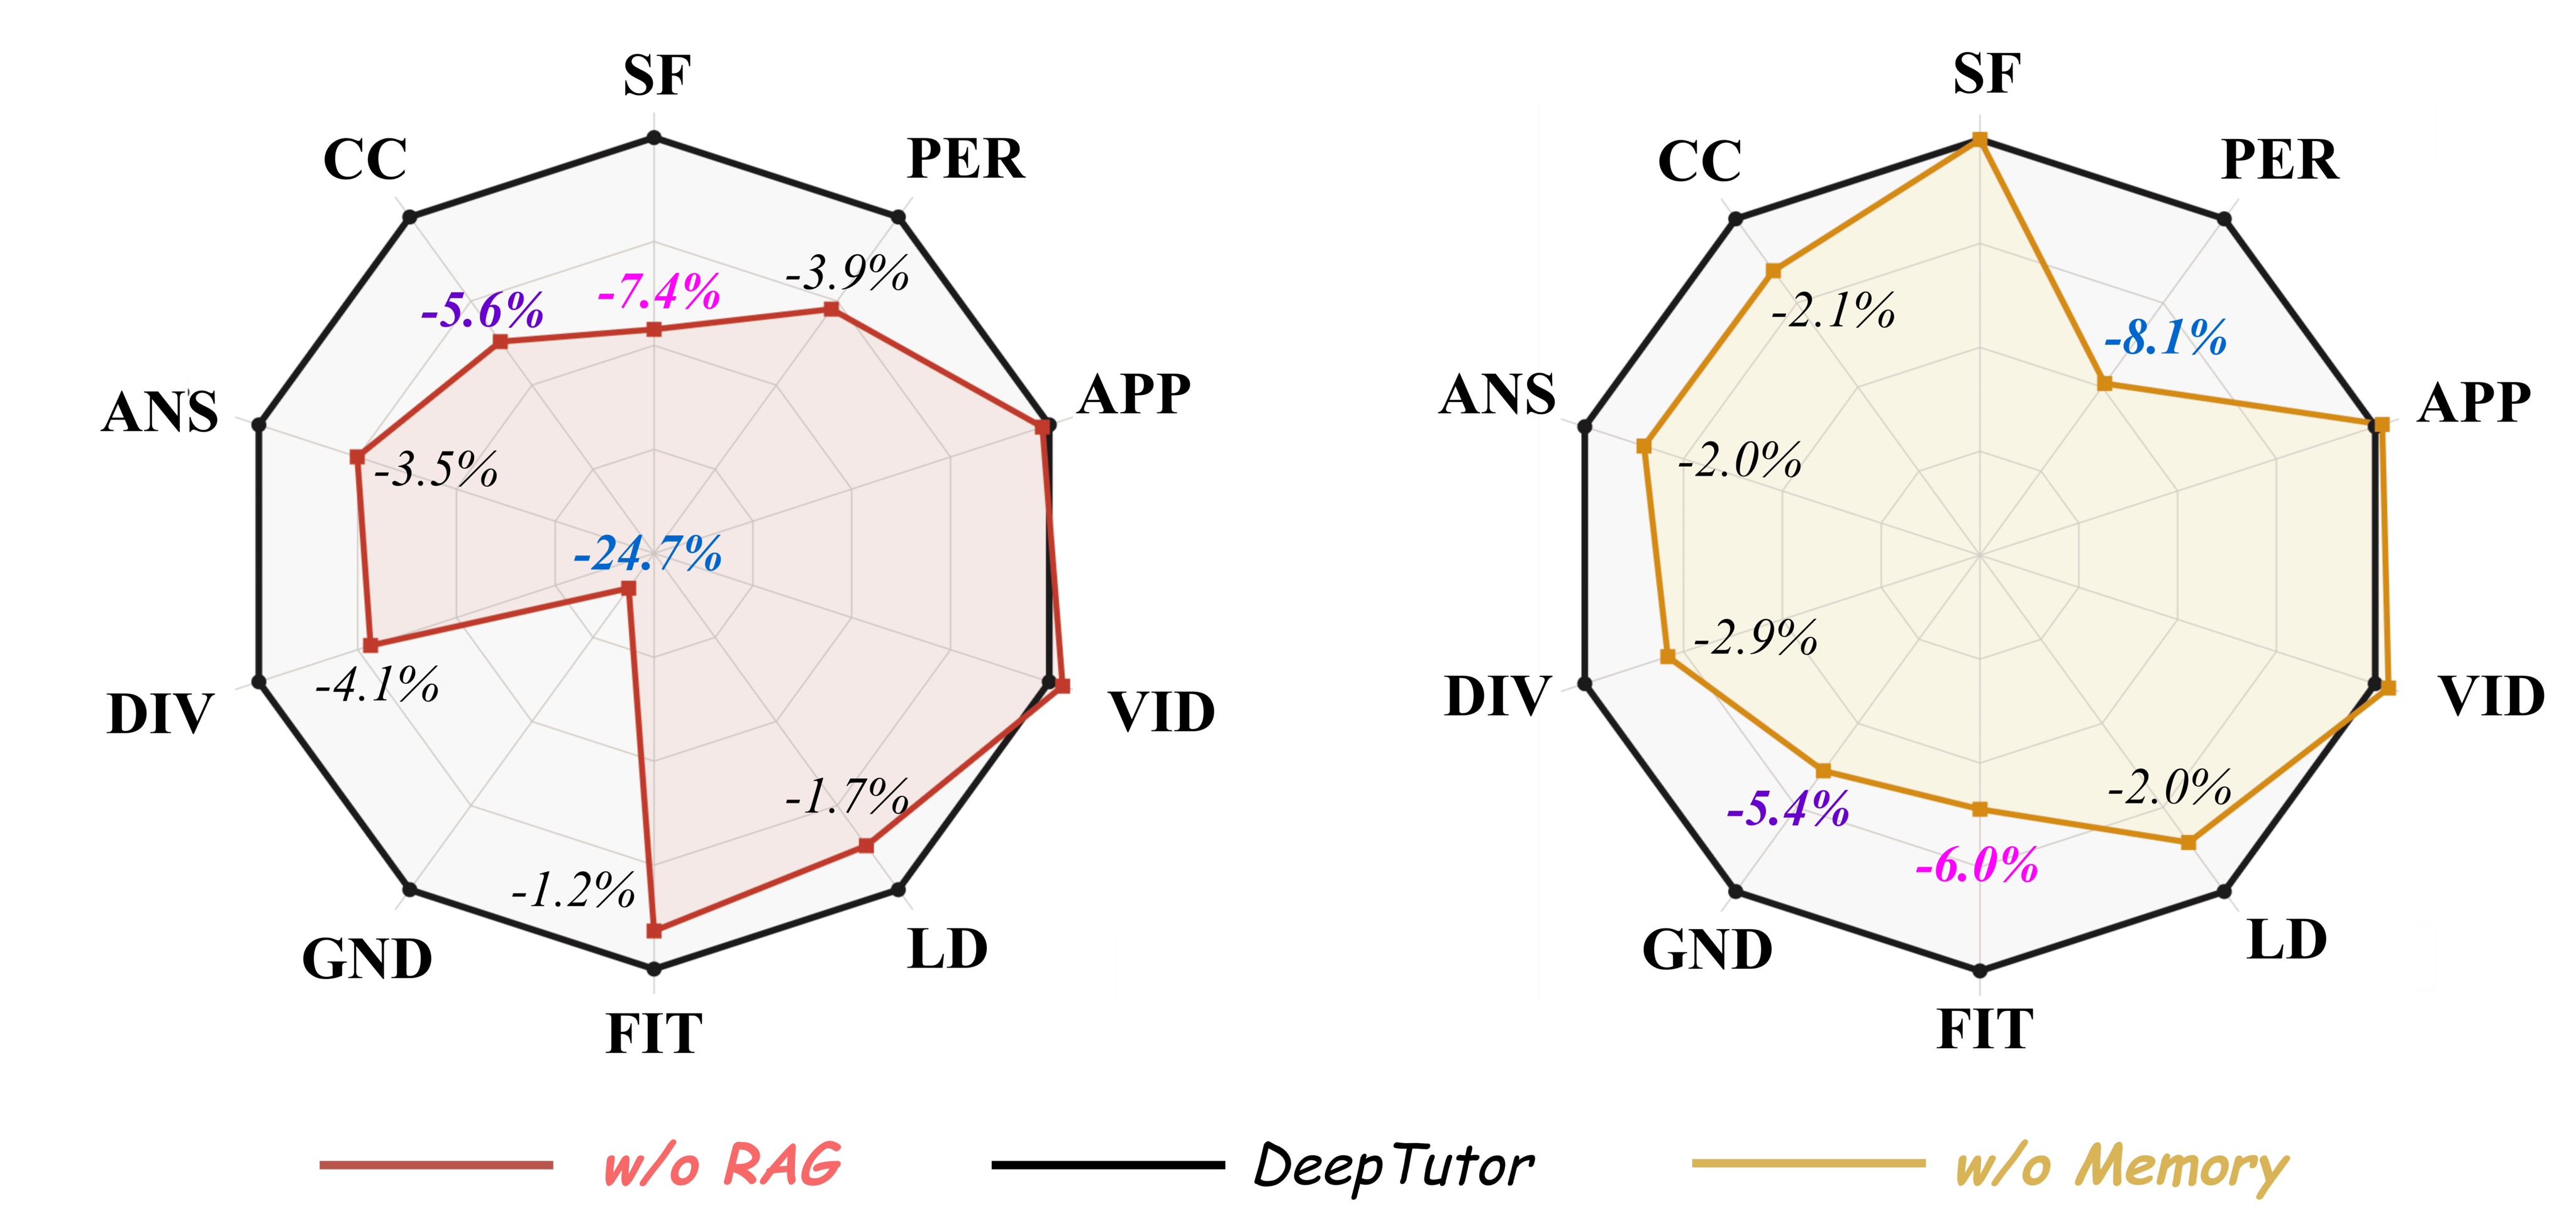
\includegraphics[width=\columnwidth]{figures/ablation-0316.png}
  \caption{Per-metric impact of removing RAG (left) and Memory (right). Black decagon: full \textsc{DeepTutor}; shaded region: ablated variant. Labels highlight the three largest drops (\textcolor[RGB]{39,123,255}{1st}, \textcolor[RGB]{255,74,234}{2nd}, \textcolor[RGB]{147,92,255}{3rd}).}
  \label{fig:ablation_radar}
\end{figure}

We ablate RAG, Memory, or both from the full pipeline (lower block of Table~\ref{tab:interactive_all}, visualized in Figure~\ref{fig:ablation_radar}).

\textbf{Removing RAG} primarily erodes content-grounding metrics.
\emph{Groundedness} suffers the steepest decline ($-$0.73), followed by \emph{Source Faithfulness} and \emph{Cross Concept}.
This is expected: without retrieval, the system loses access to the authoritative material that anchors both explanations and practice items.

\textbf{Removing Memory} instead compresses the personalization cluster.
\emph{Personalization} falls most sharply ($-$0.37), followed by \emph{Fitness} and \emph{Groundedness}.
The drop in \emph{Fitness} is particularly informative, as it confirms that learner memory is the primary signal for calibrating practice difficulty to the individual.

The two ablation patterns contract along \emph{largely complementary} axes: RAG governs \emph{what} the tutor says in terms of factual grounding, while Memory shapes \emph{how} it adapts in terms of personalization depth.
This complementarity confirms that the two components serve distinct functions and reinforces the rationale behind the hybrid personalization engine.
Even when both are removed, \textsc{DeepTutor} still outperforms all baselines by 4.82\%, indicating that the multi-stage pipeline itself contributes meaningfully beyond the personalization modules.
